\documentclass[table]{beamer}


% Setup appearance:
\usetheme{Darmstadt}
\usefonttheme[onlylarge]{structurebold}
\setbeamerfont*{frametitle}{size=\normalsize,series=\bfseries}
\setbeamertemplate{navigation symbols}{}
\addtobeamertemplate{navigation symbols}{}{%
	\usebeamerfont{footline}%
	\usebeamercolor[fg]{footline}%
	\hspace{1em}%
	\insertframenumber/\inserttotalframenumber
}
\setbeamercolor{footline}{fg=black}
% Standard packages
\usepackage[english]{babel}
\usepackage[utf8]{inputenc}
\usepackage{times}
\usepackage[T1]{fontenc}
\usepackage{ragged2e}
\usepackage{verbatim}
\usepackage{algorithm2e}
\usepackage{multirow}
\usepackage{pgffor}
\usepackage{arrayjob}
\graphicspath{{images/}}

% Setup TikZ
\usepackage{tikz}
\usetikzlibrary{arrows}
\tikzstyle{block}=[draw opacity=0.7,line width=1.4cm]


% Author, Title, etc.

\title[Block Partitioning and Perfect Phylogenies] 
{
	Improving Robustness in Social Fabric-based Cultural Algorithms
}

\author[]
{
	Bahram Zaeri\inst{1} \newline
	Advisor: Dr. Ziad Kobti\inst{1}\newline
	Internal Reader: Dr. Mehdi Kargar\inst{1}\newline
	External Reader: Dr. Kemal Tepe\inst{2}
}

\institute[Tübingen and others]
{
	\inst{1}%
	University of Windsor, School of Computer Science
	\and
	\vskip-2mm
	\inst{2}%
	University of Windsor, Dept. of Electrical and Computer Eng.
}

\date[WABI 2006]
{\textbf{Master Thesis Defence}}

\setbeamertemplate{blocks}[rounded][shadow=true]
% The main document

\newarray\meansfpso
\readarray{meansfpso}{2.138157e+08&1.352649e+04&3.064714e+02&1.583199e+03&5.015503e+02&6.009482e+02&7.042910e+02&8.203406e+02&9.036447e+02&8.964483e+04&1.106949e+03&1.300718e+03&1.623582e+03&1.601566e+03&1.609993e+03}
\newarray\meansfep
\readarray{meansfep}{2.040872e+09&3.503926e+04&3.138285e+02&3.172025e+03&5.067958e+02&6.034668e+02&7.999019e+02&5.558336e+06&9.044253e+02&5.004825e+05&1.166344e+03&1.509656e+03&3.778261e+03&1.626201e+03&2.046239e+03}
\newarray\meanpso
\readarray{meanpso}{3.048318e+08&2.302715e+04&3.067392e+02&1.366547e+03&5.015435e+02&6.017535e+02&7.119572e+02&8.529971e+02&9.035262e+02&7.352657e+04&1.105856e+03&1.282192e+03&1.634022e+03&1.607456e+03&1.825546e+03}
\newarray\meancaep
\readarray{meancaep}{3.107426e+09&7.939967e+04&3.112132e+02&2.393013e+03&5.043716e+02&6.066964e+02&8.024372e+02&5.026356e+03&9.044749e+02&1.662734e+07&1.166454e+03&6.295140e+03&3.614249e+03&1.635996e+03&2.130541e+03}
\newarray\bestsfpso
\readarray{bestsfpso}{359556.9286&10787.6651&306.2688&1443.1549&501.2390&600.8015&703.7501&816.5554&903.5440&10332.5348&1106.3587&1295.6163&1617.4672&1599.4823&1547.9172}
\newarray\bestsfep
\readarray{bestsfep}{7.555975e+07&1.196876e+04&3.138285e+02&3.172025e+03&5.067913e+02&6.023944e+02&7.999019e+02&5.558336e+06&9.044253e+02&5.004824e+05&1.166344e+03&1.393729e+03&3.778261e+03&1.626201e+03&2.046175e+03}
\newarray\bestpso
\readarray{bestpso}{102479.1580&13856.2910&305.8978&1038.6803&501.4278&601.4588&709.9928&815.2187&903.4610&7933.8017&1104.1271&1252.4376&1626.4161&1606.6267&1776.2794}
\newarray\bestcaep
\readarray{bestcaep}{2.186939e+09&3.782168e+04&3.111638e+02&2.393013e+03&5.043702e+02&6.066964e+02&8.024372e+02&8.148824e+02&9.044749e+02&1.662734e+07&1.166454e+03&6.295137e+03&3.614249e+03&1.635996e+03&2.130541e+03}
\newarray\stdsfpso
\readarray{stdsfpso}{3.645873e+08&6.525792e+03&6.619418e-01&1.425163e+02&1.903829e-01&2.992537e-01&2.108978e+00&1.119677e+01&1.084524e-01&1.987697e+05&9.061842e-01&2.087508e+01&1.151908e+01&1.754175e+00&7.597716e+01}
\newarray\stdsfep
\readarray{stdsfep}{2.940984e+09&2.180314e+05&0.000000e+00&0.000000e+00&7.606342e-03&1.013019e+00&0.000000e+00&0.000000e+00&0.000000e+00&2.716484e-01&2.996447e-04&2.199706e+02&0.000000e+00&0.000000e+00&6.373723e-01}
\newarray\stdpso
\readarray{stdpso}{4.962778e+08&8.457301e+03&5.086404e-01&2.257014e+02&1.996635e-01&2.406625e-01&1.903651e+00&5.460419e+01&9.712358e-02&9.838880e+04&9.740308e-01&5.158630e+01&7.787729e+00&7.200704e-01&9.348504e+01}
\newarray\stdcaep
\readarray{stdcaep}{2.347094e+09&2.101425e+05&5.691358e-02&0.000000e+00&1.425465e-02&1.518526e-06&2.797087e-05&1.667206e+04&0.000000e+00&0.000000e+00&0.000000e+00&2.864512e-02&0.000000e+00&0.000000e+00&0.000000e+00}

\begin{document}
\begin{frame}
	\titlepage
\end{frame}

\begin{frame}{Outline}
	\tableofcontents
\end{frame}


\section{Introduction}

\begin{frame}{What is Evolutionary Computation(EC)?}
	\begin{block}{Evolutionary Computation}
	%		\fontsize{13pt}{14pt}\selectfont
		\justifying
		An abstraction from the concepts of biological evolution and social interactions that is used to create optimization algorithms or methodologies that are used to solve problems. \cite{eiben2003introduction} EC algorithms are natural-inspired, population-based, iterational and utilize step-by-step improvement approaches.
	\end{block}
	\begin{block}{}
		\begin{itemize}
			\item Genetic Algorithm
			\item \alert{Cultural Algorithms}
			\item \alert{Particle Swarm Optimization}
			\item Ant Colony Optimization
			%\item Biologically inspired
			%\item Socially inspired
		\end{itemize}
	\end{block}
\end{frame}
	
\begin{frame}{Robustness}
	\begin{block}{Robustness in Evolutionary Algorithms}
		\begin{itemize}
				\item The ability to address a vast range of problems with particular qualities with a minimum number of adjustments.\newline
				\item Self-organized algorithms can learn and adapt themselves to different search landscapes.\newline
				\item Such strategies improve robustness in population-based algorithms.
		\end{itemize}
	\end{block}
\end{frame}
	
\begin{frame}{Social Fabric}
	\begin{block}{}
		\begin{itemize}
			\justifying
			\item Social Fabric was proposed by \cite{R:1}
			\item The Social Fabric is a dynamic information skin created by the agents interactions in a social context.
			%\item The informational skins are formed by the connectivity of each agent with other agents.
			\item These dynamic formations control the topology and type of interactions in the dynamic social sculpture. \cite{reynolds2008computing}
			%\item The purpose of the Social Fabric metaphor is to describe group behaviors and engineered emergent phenomena.
			\item Social interactions between individuals are modeled using an undirected graph $G(V;E)$ \cite{sterling2004aggregation}.
			\item In this research work, The Social Fabric approach is used to improve the search behavior of evolutionary algorithms in multi-dimensional search spaces.
		\end{itemize}
	\end{block}
\end{frame}
	
	\begin{frame}{Research Motivation}
		\begin{block}{Optimization Problems}
			\begin{itemize}
				\justifying
				\item CEC-2015 expensive optimization problem set is used to evaluate the proposed approaches. \cite{chen2014problem}
				\item It is a set of 15 real-world numerical optimization problems that was used in IEEE-CEC2015 and 2016 competitions on testing evolutionary algorithms.
				\item Because of their high dimensionality, multimodality, and copious local optima, they are suitable to inspect and compare the capabilities of evolutionary algorithms regarding robustness, scalability, adaptability, etc.
			\end{itemize}
		\end{block}
%		\begin{block}{}
%			$y=f(x\textsubscript{1}, x\textsubscript{2}, \cdots, x\textsubscript{n})$\newline
%			It aims at finding a vector $x\textup{*}$ which holds:
%			\begin{center}
%				123%$f(x\textup{*})<f(x)$ for all $x$ vectors.
%			\end{center}
%		\end{block}
	\end{frame}
	
	\begin{frame}{Reaserch Goals}
		\begin{block}{}
			\begin{itemize}
				\justifying
				\item In this research work, I am going to improve Cultural Algorithms from three aspects:
				\item Applying PSO algorithm to current Social Fabric based CAs.
				\item Introducing a Irregular Neighborhood Restructuring operator to increase the level of diversity.
				\item Improving the robustness of the Belief Space by introducing a Confidence-based knowledge source inspired from Statistics.
				\item For the comparison purpose, I am going to use CEC2015 benchmark optimization functions to compare my proposed approaches against already proposed algorithms.
			\end{itemize}
		\end{block}
	\end{frame}
	
	\section{Related Works}
	
	\begin{frame}{Related Works I}
			\begin{itemize}
				\justifying
				\item \cite{R:1} introduced the idea of Social Fabric as a new influence function in CA by deploying a social network between individuals.
				\item \cite{che2010robust} replaced the traditional idea of roulette wheel with the vector voting model to determine the controller KS in each iteration.
				\item \cite{ali2012socio} introduced the neighborhood restructuring in Social Fabric with a two-layered multi-population CA model.
				\item \cite{chen2006tribe} introduced Tribe-PSO algorithm as a multi-tribe population-based algorithm to utilize the parallel nature of evolutionary algorithms.
			\end{itemize}
	\end{frame}
	
	\begin{frame}{Related Works II}
		\begin{itemize}
			\justifying
			\item \cite{de2009heterogeneous} investigates different types of heterogeneity in PSO algorithm in three categories: neighborhood, update rule and parameters.
			\item \cite{ali2016leveraged} gives a detailed description of Social Fabric based MPCA with neighborhood restructuring. It, also, proves its optimality against different optimization algorithms based on an extended benchmark testbed.
		\end{itemize}
	\end{frame}
	
	\section{Evolutionary Computation}
	
	\begin{frame}{Biologically inspired algorithms}
		\begin{block}{}
			\begin{itemize}
			\justifying
			\item Biologically inspired algorithms try to mimic biological evolution process. \cite{man2012genetic}
			\item They comprise of a population of candidate solutions or individuals. Each individual is characterized by a set of genotypes or chromosomes. 
			\item Evolutionary operators are used to evolving the individuals such as \alert{Crossover}(exploitation) and \alert{Mutation}(exploration).
			\item In each iteration of these algorithms, a new population is generated through applying evolutionary operators on individuals of a generation.
			\end{itemize}
		\end{block}
		\begin{block}{}
			\begin{itemize}
				\item Genetic Algorithm
				\item Evolutionary Programming
				\item Genetic Programming				
			\end{itemize}
		\end{block}
	\end{frame}
	
	\begin{frame}{Socially inspired algorithms}
		\begin{block}{Swarm Intelligence}
			\justifying
			\cite{kennedy2001swarm} Socially inspired algorithms(Swarm Intelligence) utilize a population of semi-rational agents(rather than dumb individuals) that have the ability to perceive their surrounding environment and cooperate with other agents in a \alert{self-organized} manner. \newline Cooperation happens through communication. The agents communicate in two general ways: Direct and Indirect.
		\end{block}
		\begin{block}{}
			\begin{itemize}
				\item Cultural Algorithms(CA) \cite{reynolds1994introduction}
				\item Particle Swarm Optimization(PSO) \cite{clerc2010particle}
				\item Ant Colony Optmization(ACO) \cite{dorigo2006ant}
			\end{itemize}
		\end{block}
	\end{frame}
	
	\section{Cultural Algorithms}
	
	\begin{frame}{Cultural Algorithms}
		\justifying
		\begin{block}{}
		Cultural algorithms are a sort of socially motivated methods which combine biological evolution with socio cognitive concepts to give an optimization method based on dual inheritance theory. CAs are composed of three components: \alert{Population space}, \alert{Belief space} and \alert{Communication protocol}.
		\end{block}
		\begin{figure}[v]
			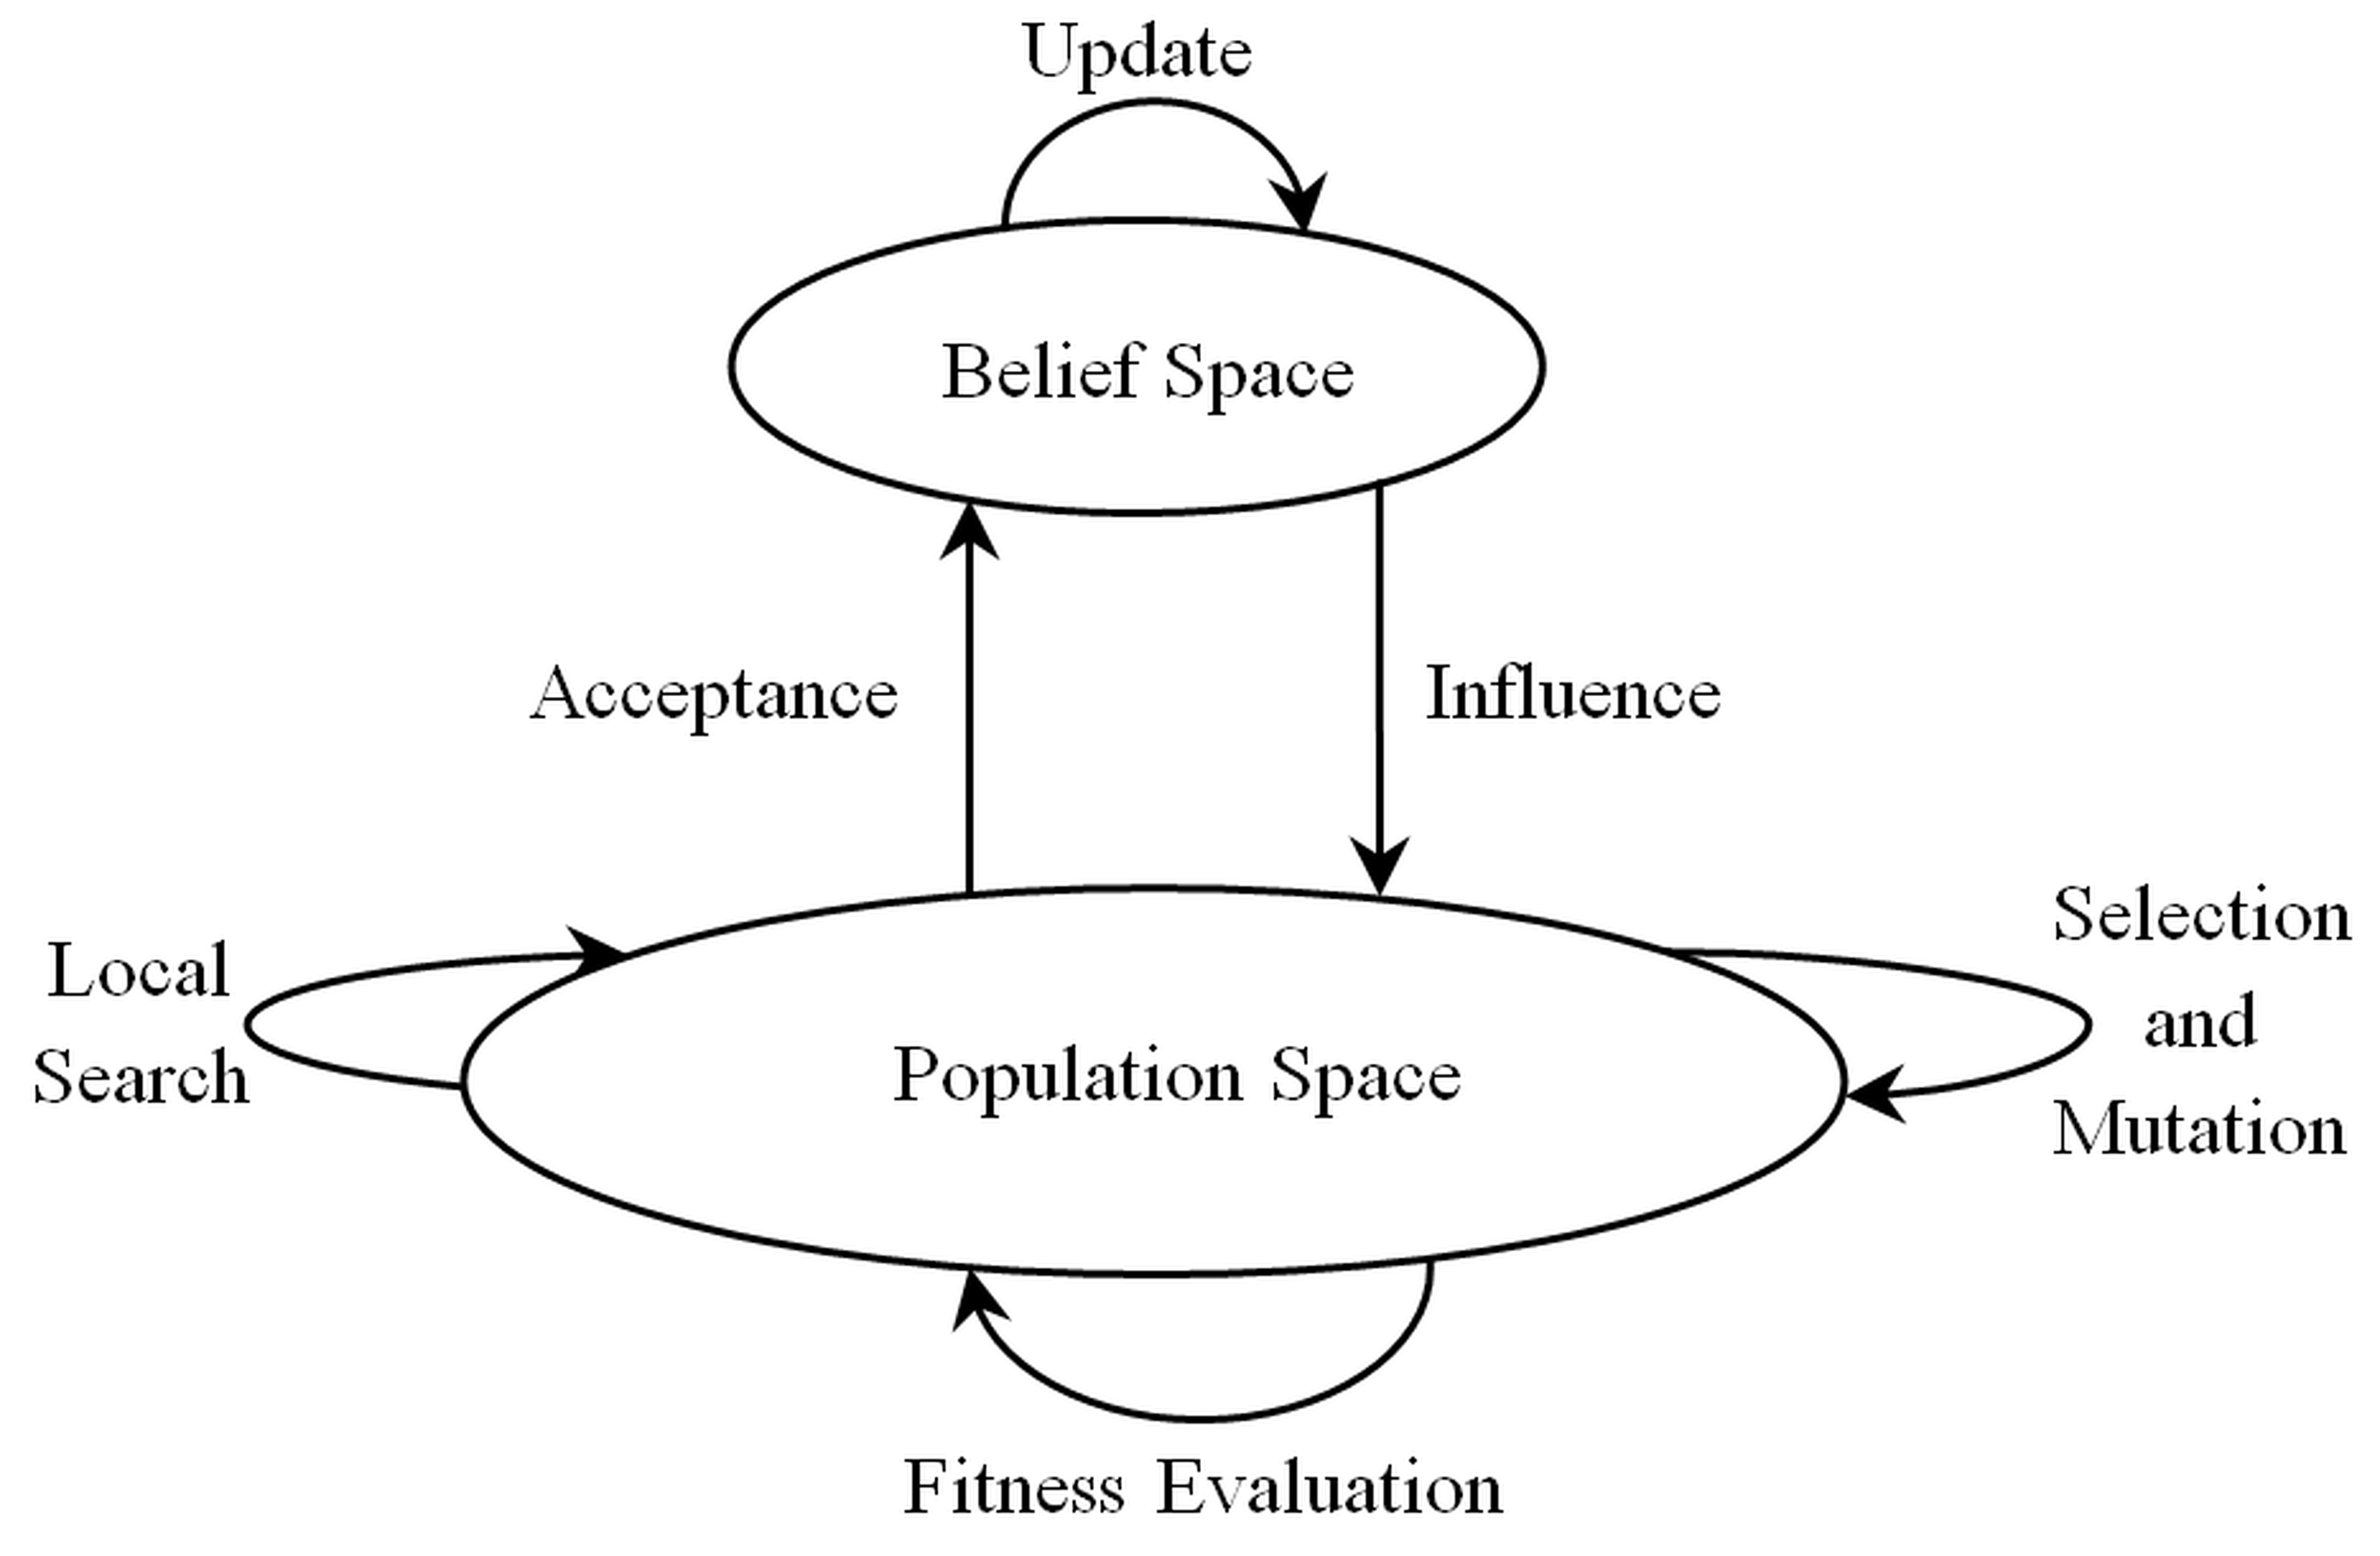
\includegraphics[scale=0.09]{CA}
			\centering
			\caption{Cultural Algorithms}
			\label{ref:CA}
		\end{figure}
	\end{frame}
	
	\begin{frame}{Cultural Algorithms}
		\begin{figure}[v]
			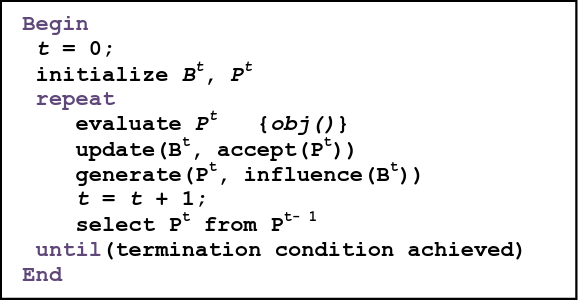
\includegraphics[scale=0.45]{capsudocode}
			\centering
			\caption{Cultural Algorithms}
			\label{ref:capsudocode}
		\end{figure}
		\begin{block}{}
			In the \alert{population-space} of CA any population-based algorithm such as GA, EP, PSO, etc. could be used.
		\end{block}
	\end{frame}
	
	\begin{frame}{Cultural Algorithms}
		\justifying
		\begin{block}{Belief Space}
			There are five types of \alert{knowledge sources} in Belief Space. The elite members of Population space are selected and sent to the Belief space to extract and utilize their knowledge through the search process. \cite{reynolds2010weaving}
		\end{block}
		\begin{block}{}
			\begin{itemize}
				\item Situational Knowledge
				\item Normative Knowledge
				\item Topographic Knowledge
				\item Domain Knowledge
				\item Historical Knowledge
			\end{itemize}
		\end{block}
	\end{frame}
	
	\begin{frame}{Cultural Algorithms}
		\begin{block}{Knowledge Sources}
			\begin{itemize}
				\item Situational: The goal of situational knowledge is to collect information from elite individuals and attempt to evolve potential solutions with this information.
				\item Normative: It is represented as a set of $n$ intervals, and each describes a promising range of good or socially acceptable solutions for each of $n$ dimensions.
			\end{itemize}
		\end{block}
		\begin{figure}[v]
			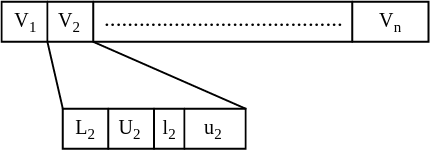
\includegraphics[scale=0.4]{normative}
			\centering
			\caption{Normative KS}
			\label{ref:normative}
		\end{figure}
	\end{frame}
	
	\begin{frame}{Cultural Algorithms}
		\begin{block}{Knowledge Sources}
			\begin{itemize}
				\item Topographic: It divides the whole landscape into cells and keeps track of the best individual in each cell. This KS is used to split the current search regions into subregions along each dimension of the problem. Each area will be divided into two new subregions in each generation of the optimization process.
			\end{itemize}
		\end{block}
		\begin{figure}[v]
			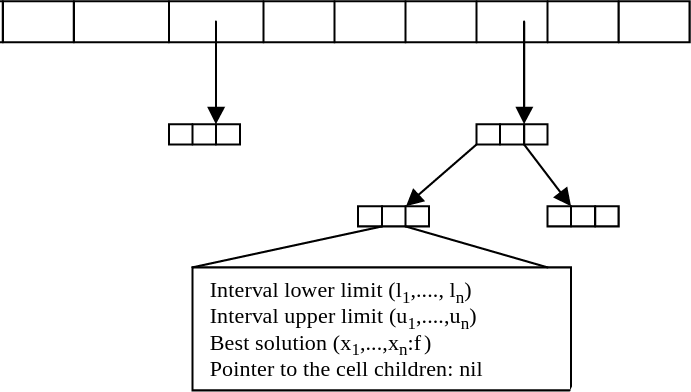
\includegraphics[scale=0.26]{topographic}
			\centering
			\caption{Topographic KS}
			\label{ref:topographic}
		\end{figure}
	\end{frame}
	
	\begin{frame}{Multi-population CA}
		\begin{block}{}
			\begin{itemize}
				\item Multi-population CAs utilize the parallel nature of evolutionary algorithms. \cite{guo2011novel}
				\item It comprises of multiple CAs that run independently.
				\item It could be heterogeneous which means any population might have different initial parameters. \cite{kobti2013heterogeneous}
			\end{itemize}
		\end{block}
		\begin{figure}[v]
			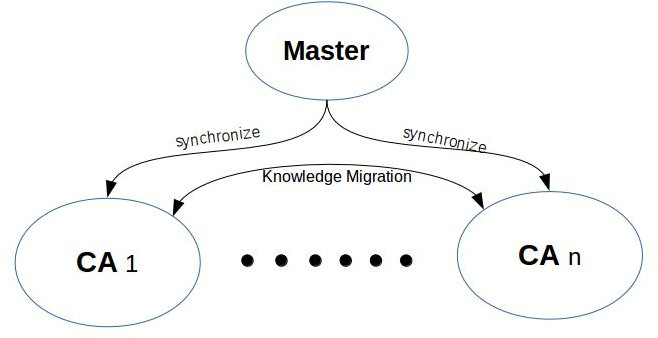
\includegraphics[scale=0.5]{mpca}
			\centering
			\caption{MPCA}
			\label{ref:mpca}
		\end{figure}
	\end{frame}
	
	\section{Social Fabric}
	
	\begin{frame}{Social Fabric}
		\begin{block}{Social Fabric based CA}
			\begin{itemize}
				\item In this model of CA, knowledge sources are allowed to influence the population through a network.
				\item Individuals might be participating in different networks which might support several layers of such networks in a hierarchical manner.
				\item The interplay of these layers and networks leads us to the concept of "\alert{Social Fabric}". \cite{reynolds2008computing}
				\item Social fabrics are formed by the connectivity of individuals together which control the topology and type of interactions in the dynamic social sculpture. 
				\item In this way, the simple interactions of individuals leads to complex community-oriented behaviors which could be expressed as an emergent phenomenon.
			\end{itemize}
		\end{block}
	\end{frame}
	
	\begin{frame}{Social Fabric}
		\begin{figure}[v]
			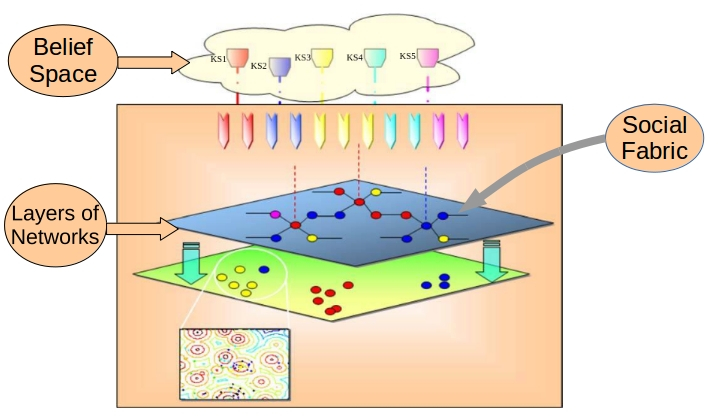
\includegraphics[scale=0.57]{socialfabric2}
			\centering
			\caption{Social Fabric: \cite{reynolds2010weaving}}
			\label{ref:socialfabric}
		\end{figure}		
	\end{frame}
	
	\begin{frame}{Social Fabric}
		\begin{block}{}
			\begin{itemize}
				\item The population is divided into multiple subgroups or \alert{tribes}. \cite{ali2016leveraged}
				\item Best(elite) individuals of each tribe form the advanced layer, while the other individuals form the rudimentary layer.
			\end{itemize}
		\end{block}
		\begin{block}{}
			\begin{itemize}
				\item The whole search process is divided into three phases:
				\item Seclusion: In this stage, all the tribes work independently without any communication.
				\item Rapport: In this stage, the tribes start to communicate, and by selecting elite members the advanced layer is formed.
				\item Cohesive: Finally, all the tribes are recombined into one population, and the search process continues until meeting some stopping criteria.
			\end{itemize}
		\end{block}
	\end{frame}
	
	\begin{frame}{Social Fabric}
		\begin{figure}[v]
			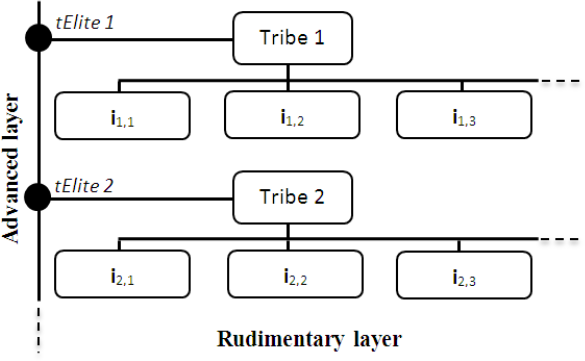
\includegraphics[scale=0.36]{twolayer}
			\centering
			\caption{Two-layered structure of the Tribal Cultural Algorithm: \cite{ali2012socio}}
			\label{ref:twolayer}
		\end{figure}		
	\end{frame}
	
	\begin{frame}{Dynamic Neighborhood Restructuring}
		\begin{block}{Strategic Restructuring}
			\begin{itemize}{}
				\item Used network topologies are regular which means all the individuals have the same neighborhood size with undirected connections.
				\item Each tribe can change its topology in the case of stagnation. 
				\item After a certain number of iterations without any progress in search behavior, the current topology is changed.
				\item The change in topology might be in either increasing the connectivity or decreasing it. %dependent upon the performance of a tribe among other tribes.
			\end{itemize}
		\end{block}
		\begin{block}{Topologies}
			\begin{itemize}
				\item Ring, Tree
				\item Mesh, Global
			\end{itemize}
		\end{block}
	\end{frame}
	
	\begin{frame}{Dynamic Neighborhood Restructuring}
		\begin{figure}[v]
			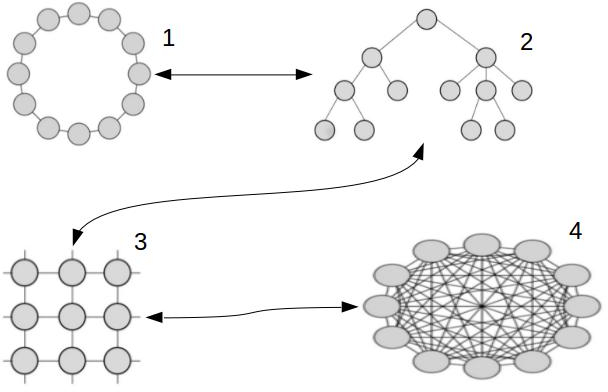
\includegraphics[scale=0.6]{restructuring}
			\centering
			\caption{Upgrading/Downgrading Strategy}
			\label{ref:restructuring}
		\end{figure}		
	\end{frame}
	
	\begin{frame}{Dynamic Neighborhood Restructuring}
		\begin{block}{}
			\eIf{tElite == recorded\_tElite}{
				\eIf{$stagnationCounter \geq triggerThreshold$}{
					$S\textsubscript{f} \gets getS\textsubscript{f}();$\newline
					$ModifyTopology(S\textsubscript{f});$\newline
					$counterStagnation \gets 0;$
				}{
					$counterStagnation \gets counterStagnation+1;$
				}
			}{
			$stagnationCounter \gets 0;$
		}
		\end{block}
	\end{frame}
	
	\begin{frame}{Social Fabric Infuence Function}
		\begin{columns}
			\begin{column}{0.6\textwidth}
				\begin{block}{}
					\begin{itemize}
						\item The social fabric represents the extent to which the influence of knowledge sources can spread through a population.
						\item Every individual is influenced by one of the KSs.
						\item Each individual receives the influencing KS of its neighbors.
						\item The KS that is used more than others will be chosen to influence the individual in the next iteration.
					\end{itemize}
				\end{block}
			\end{column}
			\begin{column}{0.4\textwidth}
				\begin{figure}[v]
					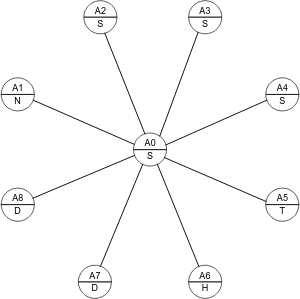
\includegraphics[scale=0.45]{votingmodel}
					\centering
					\caption{Knowledge Sources Interaction at Population Space}
					\label{ref:votingmodel}
				\end{figure}
			\end{column}
		\end{columns}
	\end{frame}
	
	\begin{frame}{Social Fabric Infuence Function}
		\begin{columns}
			\begin{column}{0.6\textwidth}
				\begin{block}{}
					\begin{itemize}
						\item Individual $A0$ has following count of votes:
						\item 3 neighbors (including itself) votes for S
						\item 2 neighbors vote for D
						\item 1 neighbors votes for T
						\item 1 neighbors votes for N
						\item 1 neighbors votes for H
					\end{itemize}
				\end{block}
				\begin{block}{}
					The Controller KS of individual A0 will be \alert{Situational} for the next iteration.
				\end{block}
			\end{column}
			\begin{column}{0.4\textwidth}
				\centering
				\begin{figure}[v]
					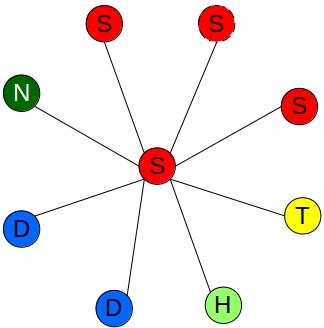
\includegraphics[scale=0.45]{votingmodel2}
					\centering
					\caption{Majority Win in Belief Space}
					\label{ref:votingmodel2}
				\end{figure}
			\end{column}
		\end{columns}
	\end{frame}
	
	\section{PSO}
	
	\begin{frame}{Particle Swarm Optimization}
		\begin{block}{}
			\justifying
			\begin{itemize}
				\item PSO works based on the theory of social learning. Individuals (Particles) move around the search space.
				\item They observe other particles and adjust their velocity and direction through the search space based on their own best experience and their neighborhood best particles. 
				\item Such behavior could be observed in natural groupings such as flocks of birds, colonies of bees, etc.
			\end{itemize}
		\end{block}
		\begin{figure}[v]
			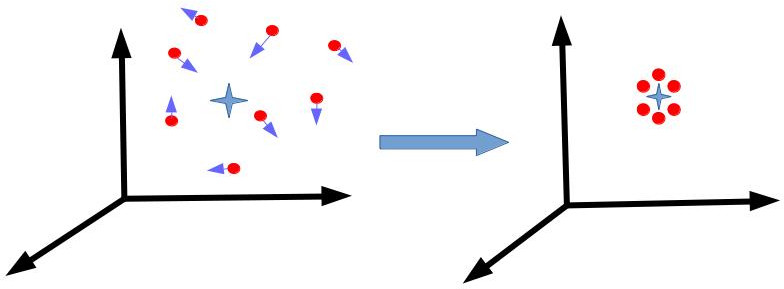
\includegraphics[scale=0.4]{pso1}
			\centering
			\caption{PSO}
			\label{ref:pso1}
		\end{figure}
	\end{frame}

	\begin{frame}{Particle Swarm Optimization}
		\begin{block}{Three principles of the Collective behavior of PSO}
			\begin{itemize}
				\item Evaluate: Learning cannot happen unless the individuals can evaluate the performance of themselves.
				\item Compare: The standards for social behaviors are set by comparison to others.
				\item Imitate: Particles improve their own performance through imitating of other better particles.
			\end{itemize}
		\end{block}
	\end{frame}

	\begin{frame}{Particle Swarm Optimization}
		\begin{block}{PSO Update Rule}
			The velocity $V\textsubscript{i}\textsuperscript{d}$ and position $X\textsubscript{i}\textsuperscript{d}$ of the $d$th dimension of the $i$th particle are updated as follows:
		\end{block}
		\begin{block}{Velocity Update}
			$V\textsubscript{i}\textsuperscript{d}(t+1) = V\textsubscript{i}\textsuperscript{d}(t) +\newline c1*rand1*(pbest\textsubscript{i}\textsuperscript{d}-X\textsubscript{i}\textsuperscript{d})+c2*rand2*(gbest\textsuperscript{d}-X\textsubscript{i}\textsuperscript{d})$
		\end{block}
		\begin{block}{Position Update}
			$X\textsubscript{i}\textsuperscript{d}(t+1)=X\textsubscript{i}\textsuperscript{d}(t)+V\textsubscript{i}\textsuperscript{d}(t)$
		\end{block}
	\end{frame}

	\begin{frame}{Particle Swarm Optimization}
		\begin{block}{Tribe-PSO}
			\begin{itemize}
				\item The whole population is divided into independent tribes. \cite{chen2006tribe}
				\item Particles fall into two layers, and the whole process consists of three phases.
				\item Best particles of each tribe form the upper layer of elites.
			\end{itemize}
		\end{block}
		\begin{figure}[v]
			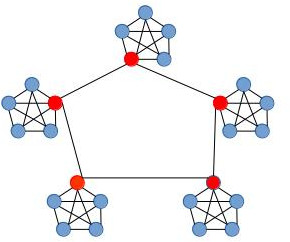
\includegraphics[scale=0.6]{tpso}
			\centering
			\caption{Tribe-PSO}
			\label{ref:tpso}
		\end{figure}		
	\end{frame}
	
	\section{Proposed Approaches}
	
	\begin{frame}{Thesis Statement}
		\begin{block}{}
			\begin{itemize}
				\justifying			
				\item In this research work, I am going to improve Cultural Algorithms from three aspects:
				\item Applying PSO algorithm to current Social Fabric based CAs.
				\item Introducing a Heterogenous Neighborhood Restructuring operator to increase the level of diversity.
				\item Improving the robustness of the Belief Space by introducing a Confidence-based knowledge source inspired from Statistics.
				\item For the comparison purpose, I am going to use CEC2015 benchmark optimization functions to compare my proposed approaches against already proposed algorithms.
			\end{itemize}
		\end{block}
	\end{frame}
		
	\begin{frame}{Proposed Approach I}
		\begin{block}{Heterogenous Neighborhood Restructuring}
			\begin{itemize}
				\item In this type of restructuring, the topology of social fabric is not considered regular.
				\item It is a directed graph which means relationships between individuals are not reciprocal.
				\item Neighborhoods are \alert{heterogenous}. Each individual has a different neighborhood size.
				\item In the standard Social Fabric, tribes' topologies change from a regular form into another in a macroscopic way in the presence of stagnation.
				\item In my proposed idea, each individual decides to increase/decrease its own neighborhood size based on its experience.
			\end{itemize}
		\end{block}
	\end{frame}
	
	\begin{frame}{Proposed Approach I}
		\begin{block}{Heterogenous Neighborhood Restructuring}
			\begin{itemize}
				\item So, the Dynamic sculpture of a Social Fabric happens at the microscopic level of each individual rather than the standard's macroscopic manner.
			\end{itemize}
		\end{block}
			\begin{figure}[v]
				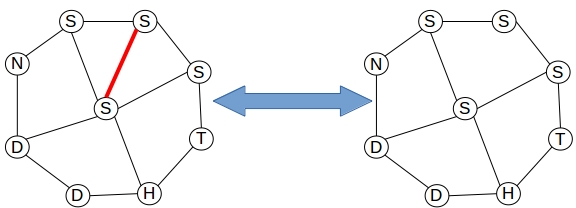
\includegraphics[scale=0.6]{heterogenous}
				\centering
				\caption{}
				\label{ref:heterogenous}
			\end{figure}				
	\end{frame}
		
	\begin{frame}{Proposed Approach I}
		\begin{block}{Pseudo-Code}
			\eIf{$fitness(x\textsubscript{i}) > bestSoFar\textsubscript{i} $}{
				\eIf{$stagnationCounter \ge TiggerThreshold$}{
					\uIf{$x\textsubscript{i} == x\textsubscript{best}$}{
						index = selected randomly from $x\textsubscript{i}$'s neighborhood\newline
						remove $x\textsubscript{index}$ from $x\textsubscript{i}$'s neighborhood
						}
					\Else{
						index = selected from $\{S - x\textsubscript{i}'s neighborhood\}$\newline
						add $x\textsubscript{index}$ to $x\textsubscript{i}$'s neighborhood
						}
						$stagnationCounter \gets 0$
					}{
					$stagnationCounter \gets stagnationCounter+1$
					}
				}{
				$stagnationCounter \gets 0$
				}
		\end{block}
	\end{frame}
		
	\begin{frame}{Proposed Approach II}
		\begin{block}{Confidence-based Normative KS}
			\begin{itemize}
				\item The standard normative KS works based on constructing a dynamic range for feasible solutions.
				\item The length of these ranges change based on the values of best individuals of each generation.
				\item Sudden changes in the values of individuals might get the normative ranges fluctuated.
				\item To avoid fluctuations, it needs to be improved regarding robustness.
				\item To do so, the concept of \alert{Confidence Interval} from Statistics could be introduced here. \cite{papoulis2002probability}
			\end{itemize}
		\end{block}
	\end{frame}
	\begin{frame}{Proposed Approach II}
		\begin{block}{Confidence-based Normative KS}
			\begin{itemize}
				\item A confidence interval provides a range of values which is likely to contain a certain percentage of a population.
				\item There is some level of arbitrariness in choosing the range size to estimate the mean.
				\item Interval estimates are often desirable because the estimate of the mean varies from sample to sample.
			\end{itemize}
		\end{block}
		\begin{block}{}
			\centering
			$(\bar{x}-q\cdot\dfrac{\sigma}{\sqrt{n}} , \bar{x}+q\cdot\dfrac{\sigma}{\sqrt{n}})$\newline
			$\bar{x}$: mean , $\sigma$: standard deviation , q: confidence coefficient
		\end{block}
	\end{frame}

	\begin{frame}{Preliminary Results I}
		\begin{center}
			\begin{table}[ht]
			\centering
			\resizebox{\textwidth}{!}{\begin{tabular}{cc|c|c|c|c|}
			\cline{3-6}
			& & SFEP & SFPSO & PSO & CAEP \\
			\hline

			\multicolumn{1}{ |c| }{\multirow{3}{*}{T1}}& 
			\multicolumn{1}{ |c| }{Mean} & \meansfep(1) & \meansfpso(1) & \meanpso(1) & \meancaep(1)\\
			\cline{2-6}
			\multicolumn{1}{ |c| }{} & \multicolumn{1}{ |c| }{Std} & \stdsfep(1) & \stdsfpso(1) & \stdpso(1) & \stdcaep(1)\\
			\cline{2-6}
			\multicolumn{1}{ |c| }{} & \multicolumn{1}{ |c| }{Best} & \bestsfep(1) & \bestsfpso(1) & \textbf{\bestpso(1)} & \bestcaep(1)\\
			\hline
			
			\multicolumn{1}{ |c| }{\multirow{3}{*}{T2}}& 
			\multicolumn{1}{ |c| }{Mean} & \meansfep(2) & \meansfpso(2) & \meanpso(2) & \meancaep(2)\\
			\cline{2-6}
			\multicolumn{1}{ |c| }{} & \multicolumn{1}{ |c| }{Std} & \stdsfep(2) & \stdsfpso(2) & \stdpso(2) & \stdcaep(2)\\
			\cline{2-6}
			\multicolumn{1}{ |c| }{} & \multicolumn{1}{ |c| }{Best} & \bestsfep(2) & \textbf{\bestsfpso(2)} & \bestpso(2) & \bestcaep(2)\\
			\hline
			
			\multicolumn{1}{ |c| }{\multirow{3}{*}{T3}}& 
			\multicolumn{1}{ |c| }{Mean} & \meansfep(3) & \meansfpso(3) & \meanpso(3) & \meancaep(3)\\
			\cline{2-6}
			\multicolumn{1}{ |c| }{} & \multicolumn{1}{ |c| }{Std} & \stdsfep(3) & \stdsfpso(3) & \stdpso(3) & \stdcaep(3)\\
			\cline{2-6}
			\multicolumn{1}{ |c| }{} & \multicolumn{1}{ |c| }{Best} & \bestsfep(3) & \bestsfpso(3) & \textbf{\bestpso(3)} & \bestcaep(3)\\
			\hline
			
			\multicolumn{1}{ |c| }{\multirow{3}{*}{T4}}& 
			\multicolumn{1}{ |c| }{Mean} & \meansfep(4) & \meansfpso(4) & \meanpso(4) & \meancaep(4)\\
			\cline{2-6}
			\multicolumn{1}{ |c| }{} & \multicolumn{1}{ |c| }{Std} & \stdsfep(4) & \stdsfpso(4) & \stdpso(4) & \stdcaep(4)\\
			\cline{2-6}
			\multicolumn{1}{ |c| }{} & \multicolumn{1}{ |c| }{Best} & \bestsfep(4) & \bestsfpso(4) & \textbf{\bestpso(4)} & \bestcaep(4)\\
			\hline
			
			\multicolumn{1}{ |c| }{\multirow{3}{*}{T5}}& 
			\multicolumn{1}{ |c| }{Mean} & \meansfep(5) & \meansfpso(5) & \meanpso(5) & \meancaep(5)\\
			\cline{2-6}
			\multicolumn{1}{ |c| }{} & \multicolumn{1}{ |c| }{Std} & \stdsfep(5) & \stdsfpso(5) & \stdpso(5) & \stdcaep(5)\\
			\cline{2-6}
			\multicolumn{1}{ |c| }{} & \multicolumn{1}{ |c| }{Best} & \bestsfep(5) & \textbf{\bestsfpso(5)} & \bestpso(5) & \bestcaep(5)\\
			\hline
			\end{tabular}}
		\end{table}
		\end{center}
	\end{frame}

	\begin{frame}{Preliminary Results II}
		\begin{center}
			\begin{table}[ht]
				\centering
				\resizebox{\textwidth}{!}{\begin{tabular}{cc|c|c|c|c|}
					\cline{3-6}
					& & SFEP & SFPSO & PSO & CAEP \\
					\hline
			\multicolumn{1}{ |c| }{\multirow{3}{*}{T6}}& 
			\multicolumn{1}{ |c| }{Mean} & \meansfep(6) & \meansfpso(6) & \meanpso(6) & \meancaep(6)\\
			\cline{2-6}
			\multicolumn{1}{ |c| }{} & \multicolumn{1}{ |c| }{Std} & \stdsfep(6) & \stdsfpso(6) & \stdpso(6) & \stdcaep(6)\\
			\cline{2-6}
			\multicolumn{1}{ |c| }{} & \multicolumn{1}{ |c| }{Best} & \bestsfep(6) & \textbf{\bestsfpso(6)} & \bestpso(6) & \bestcaep(6)\\
			\hline
			
			\multicolumn{1}{ |c| }{\multirow{3}{*}{T7}}& 
			\multicolumn{1}{ |c| }{Mean} & \meansfep(7) & \meansfpso(7) & \meanpso(7) & \meancaep(7)\\
			\cline{2-6}
			\multicolumn{1}{ |c| }{} & \multicolumn{1}{ |c| }{Std} & \stdsfep(7) & \stdsfpso(7) & \stdpso(7) & \stdcaep(3)\\
			\cline{2-6}
			\multicolumn{1}{ |c| }{} & \multicolumn{1}{ |c| }{Best} & \bestsfep(7) & \textbf{\bestsfpso(7)} & \bestpso(7) & \bestcaep(7)\\
			\hline
			
			\multicolumn{1}{ |c| }{\multirow{3}{*}{T8}}& 
			\multicolumn{1}{ |c| }{Mean} & \meansfep(8) & \meansfpso(8) & \meanpso(8) & \meancaep(8)\\
			\cline{2-6}
			\multicolumn{1}{ |c| }{} & \multicolumn{1}{ |c| }{Std} & \stdsfep(8) & \stdsfpso(8) & \stdpso(8) & \stdcaep(8)\\
			\cline{2-6}
			\multicolumn{1}{ |c| }{} & \multicolumn{1}{ |c| }{Best} & \bestsfep(8) & \bestsfpso(8) & \textbf{\bestpso(8)} & \bestcaep(8)\\
			\hline
			
			\multicolumn{1}{ |c| }{\multirow{3}{*}{T9}}& 
			\multicolumn{1}{ |c| }{Mean} & \meansfep(9) & \meansfpso(9) & \meanpso(9) & \meancaep(9)\\
			\cline{2-6}
			\multicolumn{1}{ |c| }{} & \multicolumn{1}{ |c| }{Std} & \stdsfep(9) & \stdsfpso(9) & \stdpso(9) & \stdcaep(9)\\
			\cline{2-6}
			\multicolumn{1}{ |c| }{} & \multicolumn{1}{ |c| }{Best} & \bestsfep(9) & \bestsfpso(9) & \textbf{\bestpso(9)} & \bestcaep(9)\\
			\hline
			
			\multicolumn{1}{ |c| }{\multirow{3}{*}{T10}}& 
			\multicolumn{1}{ |c| }{Mean} & \meansfep(10) & \meansfpso(10) & \meanpso(10) & \meancaep(10)\\
			\cline{2-6}
			\multicolumn{1}{ |c| }{} & \multicolumn{1}{ |c| }{Std} & \stdsfep(10) & \stdsfpso(10) & \stdpso(10) & \stdcaep(10)\\
			\cline{2-6}
			\multicolumn{1}{ |c| }{} & \multicolumn{1}{ |c| }{Best} & \bestsfep(10) & \bestsfpso(10) & \textbf{\bestpso(10)} & \bestcaep(10)\\
			\hline					
				\end{tabular}}
			\end{table}
		\end{center}
	\end{frame}

	\begin{frame}{Preliminary Results III}
		\begin{center}
			\begin{table}[ht]
				\centering
				\resizebox{\textwidth}{!}{\begin{tabular}{cc|c|c|c|c|}
						\cline{3-6}
						& & SFEP & SFPSO & PSO & CAEP \\
						\hline
			\multicolumn{1}{ |c| }{\multirow{3}{*}{T11}}& 
			\multicolumn{1}{ |c| }{Mean} & \meansfep(11) & \meansfpso(11) & \meanpso(11) & \meancaep(11)\\
			\cline{2-6}
			\multicolumn{1}{ |c| }{} & \multicolumn{1}{ |c| }{Std} & \stdsfep(11) & \stdsfpso(11) & \stdpso(11) & \stdcaep(11)\\
			\cline{2-6}
			\multicolumn{1}{ |c| }{} & \multicolumn{1}{ |c| }{Best} & \bestsfep(11) & \bestsfpso(11) & \textbf{\bestpso(11)} & \bestcaep(11)\\
			\hline
			
			\multicolumn{1}{ |c| }{\multirow{3}{*}{T12}}& 
			\multicolumn{1}{ |c| }{Mean} & \meansfep(12) & \meansfpso(12) & \meanpso(12) & \meancaep(12)\\
			\cline{2-6}
			\multicolumn{1}{ |c| }{} & \multicolumn{1}{ |c| }{Std} & \stdsfep(12) & \stdsfpso(12) & \stdpso(12) & \stdcaep(12)\\
			\cline{2-6}
			\multicolumn{1}{ |c| }{} & \multicolumn{1}{ |c| }{Best} & \bestsfep(12) & \bestsfpso(12) & \textbf{\bestpso(12)} & \bestcaep(12)\\
			\hline
			
			\multicolumn{1}{ |c| }{\multirow{3}{*}{T13}}& 
			\multicolumn{1}{ |c| }{Mean} & \meansfep(13) & \meansfpso(13) & \meanpso(13) & \meancaep(13)\\
			\cline{2-6}
			\multicolumn{1}{ |c| }{} & \multicolumn{1}{ |c| }{Std} & \stdsfep(13) & \stdsfpso(13) & \stdpso(13) & \stdcaep(13)\\
			\cline{2-6}
			\multicolumn{1}{ |c| }{} & \multicolumn{1}{ |c| }{Best} & \bestsfep(13) & \textbf{\bestsfpso(13)} & \bestpso(13) & \bestcaep(13)\\
			\hline
			
			\multicolumn{1}{ |c| }{\multirow{3}{*}{T14}}& 
			\multicolumn{1}{ |c| }{Mean} & \meansfep(14) & \meansfpso(14) & \meanpso(14) & \meancaep(14)\\
			\cline{2-6}
			\multicolumn{1}{ |c| }{} & \multicolumn{1}{ |c| }{Std} & \stdsfep(14) & \stdsfpso(14) & \stdpso(14) & \stdcaep(14)\\
			\cline{2-6}
			\multicolumn{1}{ |c| }{} & \multicolumn{1}{ |c| }{Best} & \bestsfep(14) & \textbf{\bestsfpso(14)} & \bestpso(14) & \bestcaep(14)\\
			\hline
			
			\multicolumn{1}{ |c| }{\multirow{3}{*}{T15}}& 
			\multicolumn{1}{ |c| }{Mean} & \meansfep(15) & \meansfpso(15) & \meanpso(15) & \meancaep(15)\\
			\cline{2-6}
			\multicolumn{1}{ |c| }{} & \multicolumn{1}{ |c| }{Std} & \stdsfep(15) & \stdsfpso(15) & \stdpso(15) & \stdcaep(15)\\
			\cline{2-6}
			\multicolumn{1}{ |c| }{} & \multicolumn{1}{ |c| }{Best} & \bestsfep(15) & \textbf{\bestsfpso(15)} & \bestpso(15) & \bestcaep(15)\\
			\hline
				\end{tabular}}
			\end{table}
		\end{center}
	\end{frame}

	\section{TimeLine}

	\begin{frame}{}
		\begin{figure}
			\caption{TimeLine}
			\centering
			\resizebox{\linewidth}{!}{% Resize table to fit within
				
				
\begin{tikzpicture}[]
				%draw horizontal line
				\draw (0,0) -- (41/1.7,0);
				%draw vertical lines
				\foreach \x in {0, 15, 30, 41}{%, 29, 36, 41
					\draw (\x/1.7,3pt) -- (\x/1.7,-3pt);
				}
				%draw nodes
				\draw (0,0) node[below=3pt] { Implementing the algorithms } node[above=3pt] { Oct 31 2016  };
				\draw (15/1.7,0) node[below=3pt] { Writing the thesis } node[above=3pt] {  Nov 30 2014  };
				\draw (30/1.7,0) node[below=3pt] { Prepraing the papers } node[above=3pt] { Dec 31 2016  };
				\draw (41/1.7,0) node[below=3pt] { Final Defence } node[above=3pt] { Jan 10 2017  };
				\end{tikzpicture}
			}
			\label{fig:time_line}
		\end{figure}
	\end{frame}

	\begin{frame}[allowframebreaks]
		\frametitle{References}
		\fontsize{6pt}{3pt}
		\bibliographystyle{apalike}
		\bibliography{beamersample}
	\end{frame}
\end{document}